\documentclass[9pt,twocolumn,twoside]{osajnl}

\journal{jocn} 

% See template introduction for guidance on setting shortarticle option
\setboolean{shortarticle}{false}
% true = letter / tutorial
% false = research / review article
% (depending on journal).

\title{\LaTeX\  template for preparing a research article for submission to the \emph{Journal of Optical Communications and Networking}}

\author[1,2,3]{Author One}
\author[2,*]{Author Two}
\author[1]{Author Three}

\affil[1]{Publications Department, The Optical Society (OSA), 2010 Massachusetts Avenue NW, Washington D.C., 20036, USA}
\affil[2]{School of Science, University of Technology, 2000 J St. NW, Washington DC, 20036, USA}
\affil[3]{School of Optics, University of Technology, 2000 J St. NW, Washington DC, 20036, USA}

\affil[*]{Corresponding author: email@my-email.com}

%% To be edited by editor
% \dates{Compiled \today}

%\ociscodes{(140.3490) Lasers, distributed feedback; (060.2420) Fibers, polarization-maintaining;(060.3735) Fiber Bragg gratings.}

%% To be edited by editor
% \doi{\url{http://dx.doi.org/10.1364/XX.XX.XXXXXX}}

\begin{abstract}
JOCN article style and format is being updated to conform to OSA journal style and format. This new template is now required for preparing a research article for submission to the \emph{Journal of Optical Communications and Networking}. Consult the \href{http://www.opticsinfobase.org/submit/style/}{OSA Author Style Guide} for general information about manuscript preparation. Please note that OSA is no longer using OCIS codes.  
\end{abstract}

\setboolean{displaycopyright}{true}

\begin{document}

\maketitle

\section{Introduction}
This  template is designed to assist with creating an article to submit to the \emph{Journal of Optical Communications and Networking}. See the OSA's \href{http://www.opticsinfobase.org/submit/style/}{Style Guide} and \href{http://www.opticsinfobase.org/submit/templates/}{Manuscript Templates} pages for more details.

If you have a question while using this template on {Overleaf}, please use the help menu (``?'') on the top bar to search for help or ask us a question using our \href{https://www.overleaf.com/contact}{contact form}.

\section{Examples of Article Components}
\label{sec:examples}

The sections below show examples of different article components.

\section{Figures and Tables}

It is not necessary to place figures and tables at the back of the manuscript. Figures and tables should be sized as they are to appear in the final article. Do not include a separate list of figure captions and table titles.

Figures and Tables should be labelled and referenced in the standard way using the \verb|\label{}| and \verb|\ref{}| commands.

\subsection{Sample Figure}

Figure \ref{fig:falsecolor} shows an example figure.

\begin{figure}[htbp]
\centering
\fbox{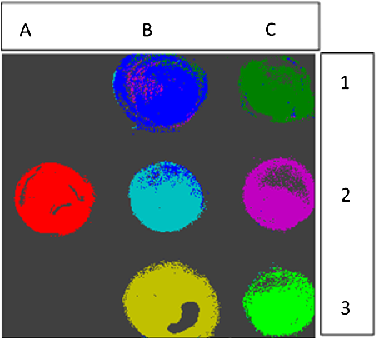
\includegraphics[width=.8\linewidth]{sample}}
\caption{False-color image, where each pixel is assigned to one of seven reference spectra.}
\label{fig:falsecolor}
\end{figure}

\subsection{Author Photographs}
Author photographs. The final printed size of an author photograph is exactly 1 inch wide by 1 1/4 inches long (6 picas × 7 1/2 picas). Please ensure that the author photographs you submit are proportioned similarly.

\subsection{Sample Table}

Table \ref{tab:shapefunctions} shows an example table.

\begin{table}[htbp]
\centering
\caption{\bf Shape Functions for Quadratic Line Elements}
\begin{tabular}{ccc}
\hline
local node & $\{N\}_m$ & $\{\Phi_i\}_m$ $(i=x,y,z)$ \\
\hline
$m = 1$ & $L_1(2L_1-1)$ & $\Phi_{i1}$ \\
$m = 2$ & $L_2(2L_2-1)$ & $\Phi_{i2}$ \\
$m = 3$ & $L_3=4L_1L_2$ & $\Phi_{i3}$ \\
\hline
\end{tabular}
  \label{tab:shapefunctions}
\end{table}

\section{Sample Equation}

Let $X_1, X_2, \ldots, X_n$ be a sequence of independent and identically distributed random variables with $\text{E}[X_i] = \mu$ and $\text{Var}[X_i] = \sigma^2 < \infty$, and let
\begin{equation}
S_n = \frac{X_1 + X_2 + \cdots + X_n}{n}
      = \frac{1}{n}\sum_{i}^{n} X_i
\label{eq:refname1}
\end{equation}
denote their mean. Then as $n$ approaches infinity, the random variables $\sqrt{n}(S_n - \mu)$ converge in distribution to a normal $\mathcal{N}(0, \sigma^2)$.

\section{Sample Algorithm}

Algorithms can be included using the commands as shown in algorithm \ref{alg:euclid}.

\begin{algorithm}
\caption{Euclid’s algorithm}\label{alg:euclid}
\begin{algorithmic}[1]
\Procedure{Euclid}{$a,b$}\Comment{The g.c.d. of a and b}
\State $r\gets a\bmod b$
\While{$r\not=0$}\Comment{We have the answer if r is 0}
\State $a\gets b$
\State $b\gets r$
\State $r\gets a\bmod b$
\EndWhile\label{euclidendwhile}
\State \textbf{return} $b$\Comment{The gcd is b}
\EndProcedure
\end{algorithmic}
\end{algorithm}

\section{Supplemental Material}

Consult the Author Guidelines for Supplementary Materials in OSA Journals for details on accepted types of materials and instructions on how to cite them.
All materials must be associated with a figure, table, or equation or be referenced in the results section of the manuscript.
(1) 2D and 3D image files and video must be labeled “Visualization,” not “Movie,” “Video,” “Figure,” etc.
(2) Machine-readable data (for example, csv files) must be labeled  “Data File.”  Number data files and visualizations consecutively, e.g., “Visualization 1, Visualization 2….”
(3) Large datasets or code files must be placed in an open, archival database.  Such items should be mentioned in the text as either “Dataset” or “Code,” as appropriate, and also be cited in the references list.  For example, “see Dataset 1 (Ref. [1]) and Code 1 (Ref [2]).” Here are examples of the references:

\subsection{Sample Dataset Citation}

1. M. Partridge, "Spectra evolution during coating," figshare (2014) [retrieved 13 May 2015], http://dx.doi.org/10.6084/m9.figshare.1004612.

\subsection{Sample Code Citation}

2. C. Rivers, "Epipy: Python tools for epidemiology," (figshare, 2014) [retrieved 13 May 2015], http://dx.doi.org/10.6084/m9.figshare.1005064.

\section{Funding and Acknowledgments}

Formal funding sources should be listed in a separate paragraph block before any other acknowledgment information. Funding sources and any associated grant numbers should match the information entered into the Prism manuscript system. Funders should be listed without any introductory language or use of labels (do not use labels such as “grant no.”). The acknowledgments may contain any information that is not related to funding. Here is an example:

\section*{Funding}National Science Foundation (NSF) (1263236, 0968895, 1102301); The 863 Program (2013AA014402).


\section*{Acknowledgments}The authors thank H. Haase, C. Wiede, and J. Gabler for technical support.

\section{References}

Full references (to aid the editor and reviewers) must be included. This will be produced automatically if you are using a .bib file.

\bigskip
\noindent Add citations manually or use BibTeX. See \cite{Chitimalla:17,Wen:16}.

% Bibliography
\bibliography{sample}

%Manual citation list
%\begin{thebibliography}{1}
%\bibitem{Zhang:14}
%Y.~Zhang, S.~Qiao, L.~Sun, Q.~W. Shi, W.~Huang, %L.~Li, and Z.~Yang,
 % \enquote{Photoinduced active terahertz metamaterials with nanostructured
  %vanadium dioxide film deposited by sol-gel method,} Opt. Express \textbf{22},
  %11070--11078 (2014).
%\end{thebibliography}




% JOCN authors may include their biographies and photos. This section is not required 

 \section*{Author Biographies}

\setlength\intextsep{0pt}

\begin{wrapfigure}{L}{0.21\textwidth}

\includegraphics[width=0.20\textwidth]{johnsmith}
\end{wrapfigure}
\paragraph{}
\noindent \textbf{First A. Author} (M’76–SM’81–F’87) and the other authors may include biographies at the end of regular papers. This author became a Member (M) of IEEE in 1976, a Senior Member (SM) in 1981, and a Fellow (F) in 1987. The first paragraph may contain a place and/or date of birth (list place, then date). Next, the author’s educational background is listed. The degrees should be listed with type of degree in what field, which institution, city, state, and country, and year degree was earned. The author’s major field of study should be lower-cased.
  
The second paragraph uses the pronoun of the person (he or she) and not the author’s last name. It lists military and work experience, including summer and fellowship jobs. Job titles are capitalized. The current job must have a location; previous positions may be listed without one. Information concerning previous publications may be included. Try not to list more than three books or published articles. The format for listing publishers of a book within the biography is: title of book (city, state: publisher name, year) similar to a reference. Current and previous research interests end the paragraph.

The third paragraph begins with the author’s title and last name (e.g., Dr. Smith, Prof. Jones, Mr. Kajor, Ms. Hunter). List any memberships in professional societies. Finally, list any awards and work for committees and publications.  If a photograph is provided, the biography will be indented around it. The photograph is placed at the top left of the biography. Personal hobbies will be deleted from the biography.\\

  \begin{wrapfigure}{L}{0.21\textwidth}
     
\includegraphics[width=0.2\textwidth]{alicesmith}
   \end{wrapfigure}
   \noindent
   \textbf{Alice Smith} received her BSc (Mathematics) in 2000 from The University of Maryland. Her research interests also include lasers and optics.\\
  
\end{document}
